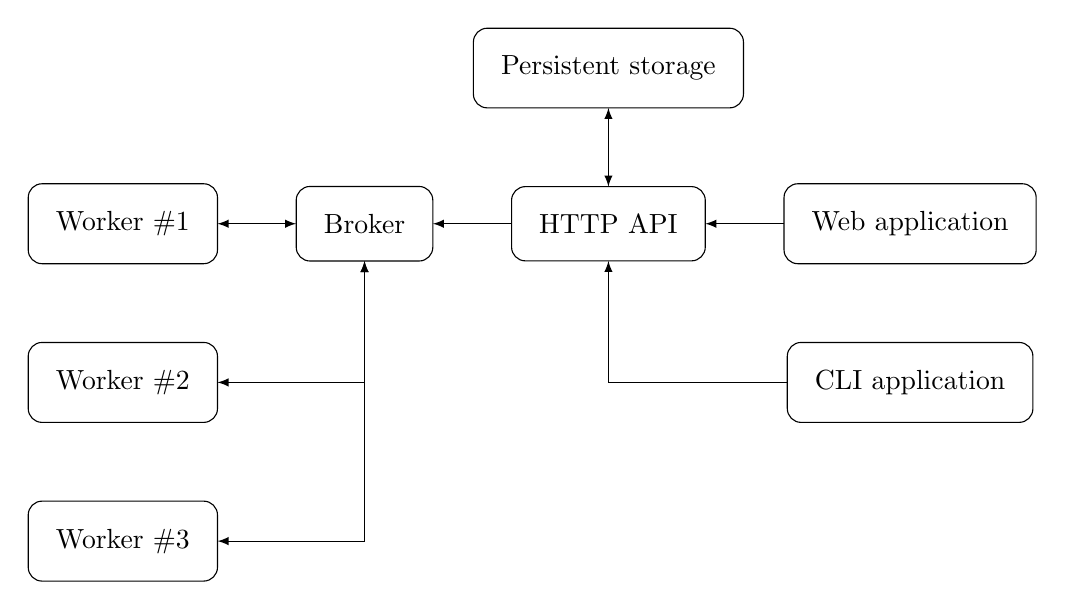
\begin{tikzpicture}[every text node part/.style={align=center}]
\usetikzlibrary{positioning}
\usetikzlibrary{fit}

\tikzstyle{bordered} = [rounded corners=5pt,rectangle,draw,outer sep=0,inner sep=10,minimum size=10]
\tikzstyle{arrow} = [draw,-latex]
\tikzstyle{doublearrow} = [draw,latex-latex]

\node [bordered] (broker) {Broker};
\node [bordered, right=of broker] (api) {HTTP API};

\node [bordered, above=of api] (storage) {Persistent storage};

\node [bordered, left=of broker] (worker_1) {Worker \#1};
\node [bordered, left=of broker, below=of worker_1] (worker_2) {Worker \#2};
\node [bordered, left=of broker, below=of worker_2] (worker_3) {Worker \#3};

\node [bordered, right=of api] (web_client) {Web application};
\node [bordered, right=of api, below=of web_client] (cli_client) {CLI application};

\path[doublearrow] (worker_1) -- (broker);
\path[doublearrow] (worker_2) -| (broker);
\path[doublearrow] (worker_3) -| (broker);

\path[arrow] (api) -- (broker);
\path[doublearrow] (api) -- (storage);

\path[arrow] (web_client) -- (api);
\path[arrow] (cli_client) -| (api);
\end{tikzpicture}
